\documentclass[twocolumn,a4paper,12pt]{article}
\usepackage{graphicx}
\begin{document}

\title{Exponential function}
\author{Wikipedia and Frederikke Vorgod}
\date{02-03-2022}
\maketitle
\section{Introduction}
The exponential function is a mathematical Function 
denoted by $f(x)=\exp(x)$ or $e^x$ (where the argument $x$ 
is written as an exponentiation). It can be defined in 
Characterizations of the exponential function several equivalent ways. 
Its ubiquitous occurrence in pure mathematics and applied mathematics 
led mathematician Walter Rudin to opine that the exponential function is 
"the most important function in mathematics"
Its value at $1$, $e = \exp(1)$ is a mathematical constant
called Euler's number. \

The graph of 
$y=e^{x}$ is upward-sloping, and increases faster as x increases. The graph always lies above the x-axis, but becomes arbitrarily close to it for large negative x; thus, the x-axis is a horizontal asymptote. The equation \ref{eq:wik} 
means that the slope of the tangent to the graph at each point is equal to its y-coordinate at that point.
\begin{equation}\label{eq:wik}
	\frac{d}{dx}e^x = e^x
\end{equation}

To implement this function, we use the following code shown in figure \ref{fig:code_exp}. 
If the argument is below $0$ it will return $1/e^x$ equivalent to $e^{-x}$. If, however, 
the argument is larger than $0$ 
and then finally returns the first few terms of the defition of the exponential function, given by
the power series in equation \ref{eq:def}

\begin{equation}\label{eq:def}
    \exp x := \sum_{k = 0}^{\infty} \frac{x^k}{k!} = 1 + x + \frac{x^2}{2} + \frac{x^3}{6} + \frac{x^4}{24} + \cdots
\end{equation}

We can now test this implementation by plotting it against known table values. This is done in \ref{fig:plot}. 
It works wooho!

\begin{figure}[b]\label{fig:code_exp}
    \includegraphics[width=\linewidth]{code_exp.png}
    \caption{Code used to implement exponential function}
\end{figure}



\begin{figure}[t]\label{fig:plot}
    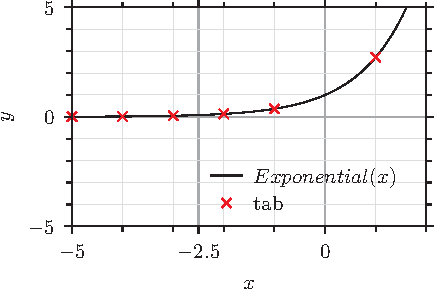
\includegraphics{exp_pyx.pdf}
    \caption{plot of the exponential function made by the code.}
\end{figure}

\end{document}
